%%%%%%%%%%%%%%%%%%%%%%%%%%%%%%%%%%%%%%%%%
% Beamer Presentation
% LaTeX Template
% Version 1.0 (10/11/12)
%
% This template has been downloaded from:
% http://www.LaTeXTemplates.com
%
% License:
% CC BY-NC-SA 3.0 (http://creativecommons.org/licenses/by-nc-sa/3.0/)
%
%%%%%%%%%%%%%%%%%%%%%%%%%%%%%%%%%%%%%%%%%

%----------------------------------------------------------------------------------------
%	PACKAGES AND THEMES
%----------------------------------------------------------------------------------------

\documentclass{beamer}
\usepackage[utf8]{inputenc}

\mode<presentation> {

% The Beamer class comes with a number of default slide themes
% which change the colors and layouts of slides. Below this is a list
% of all the themes, uncomment each in turn to see what they look like.

% \usetheme{default}
% \usetheme{AnnArbor}
%\usetheme{Antibes}
%\usetheme{Bergen}
% \usetheme{Berkeley}
%\usetheme{Berlin}
%\usetheme{Boadilla}
% \usetheme{CambridgeUS}
% \usetheme{Copenhagen}
%\usetheme{Darmstadt}
% \usetheme{Dresden}
% \usetheme{Frankfurt}
% \usetheme{Goettingen}
% \usetheme{Hannover}
%\usetheme{Ilmenau}
% \usetheme{JuanLesPins}
% \usetheme{Luebeck}
\usetheme{Madrid}
% \usetheme{Malmoe}
%\usetheme{Marburg}
% \usetheme{Montpellier}
% \usetheme{PaloAlto}
% \usetheme{Pittsburgh}
% \usetheme{Rochester}
% \usetheme{Singapore}
%\usetheme{Szeged}
%\usetheme{Warsaw}

% As well as themes, the Beamer class has a number of color themes
% for any slide theme. Uncomment each of these in turn to see how it
% changes the colors of your current slide theme.

%\usecolortheme{albatross}
%\usecolortheme{beaver}
%\usecolortheme{beetle}
%\usecolortheme{crane}
% \usecolortheme{dolphin}
%\usecolortheme{dove}
%\usecolortheme{fly}
%\usecolortheme{lily}
% \usecolortheme{orchid}
%\usecolortheme{rose}
%\usecolortheme{seagull}
%\usecolortheme{seahorse}
%\usecolortheme{whale}
%\usecolortheme{wolverine}

%\setbeamertemplate{footline} % To remove the footer line in all slides uncomment this line
%\setbeamertemplate{footline}[page number] % To replace the footer line in all slides with a simple slide count uncomment this line

%\setbeamertemplate{navigation symbols}{} % To remove the navigation symbols from the bottom of all slides uncomment this line
}

\usepackage{graphicx} % Allows including images
    \graphicspath{{../../graphics/}} % Set default directory for embedded images 
\usepackage{booktabs} % Allows the use of \toprule, \midrule and \bottomrule in tables

\usepackage{verbatim}

\usepackage{xeCJK}    % 允许使用中文
    \xeCJKsetup{PunctStyle=kaiming}  % 设置中文标点符号,开明式
    \setCJKfamilyfont{yh}{Microsoft YaHei} % 设置中文字体为微软雅黑
\usepackage{zhnumber} % 日期等匹配中文

%----------------------------------------------------------------------------------------
%	TITLE PAGE
%----------------------------------------------------------------------------------------

\title[《机器人学导论》课程设计]{《机器人学导论》课程设计} % The short title appears at the bottom of every slide, the full title is only on the title page

\author{肖书奇} % Your name
\institute[18级自动化三班] % Your institution as it will appear on the bottom of every slide, may be shorthand to save space
{
\\ % Your institution for the title page
\medskip
% \textit{john@smith.com} % Your email address
}

% \date{\today} % Date, can be changed to a custom date
\date{\zhtoday} % Date, can be changed to a custom date

\begin{document}

\begin{frame}
    \titlepage % Print the title page as the first slide
\end{frame}

\begin{frame}
    \frametitle{目录} % Table of contents slide, comment this block out to remove it
    \tableofcontents % Throughout your presentation, if you choose to use \section{} and \subsection{} commands, these will automatically be printed on this slide as an overview of your presentation
\end{frame}

%----------------------------------------------------------------------------------------
%	PRESENTATION SLIDES
%----------------------------------------------------------------------------------------

%------------------------------------------------

\section{任务分析}
\subsection{堆积木}

\begin{frame}
    \frametitle{堆积木}
    \begin{columns}[onlytextwidth,T]
        \column{\dimexpr\linewidth-50mm}
        \begin{itemize}
            \item Intel Realsense D455相机
            \item QKM SI7400开放式六轴串联机器人
        \end{itemize}
        \vspace*{2cm}
        \par 要求:
        \begin{enumerate}
            \item 积木随机散落桌面上;
            \item 可以指定积木的搭建方法;
            \item 越高越好,越快越好。
        \end{enumerate}
        \column{45mm}
        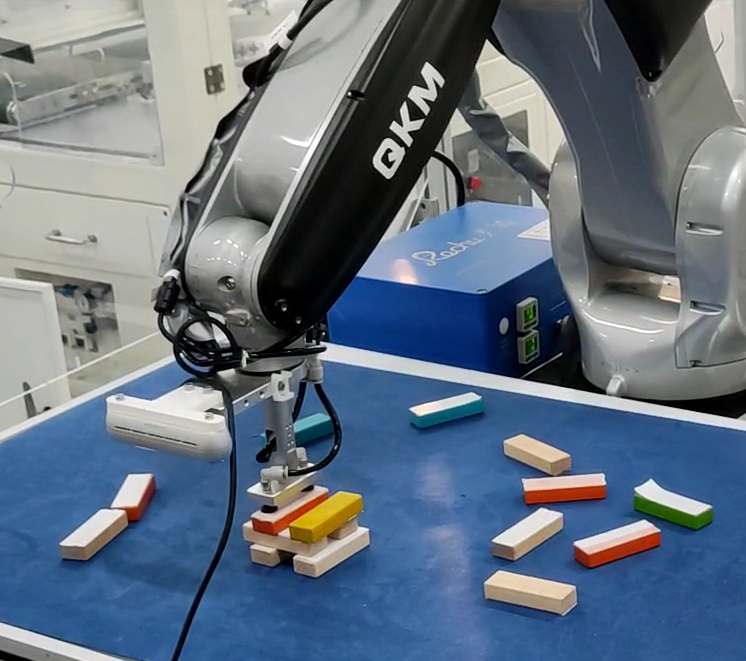
\includegraphics[width=38mm]{试验.png}
    \end{columns}
\end{frame}

%------------------------------------------------

\subsection{子任务与解决方案}

%------------------------------------------------

\begin{frame}
    \frametitle{子任务与解决方案}
    \centering
    \begin{tabular}{ccc}
        \toprule
          & 子任务   & 解决方案                               \\
        \midrule
        1 & 手眼标定 & 迭代法解Perspective-n-Point问题        \\
        2 & 物体识别 & HSV颜色分割与矩形识别                  \\
        3 & 逆运动学 & 旋量理论与Paden-Kahan子问题求解        \\
        4 & 路径规划 & 凸优化求解含约束条件的几何中点         \\
        5 & 轨迹规划 & 操作空间下梯形速度规划                 \\
        6 & 网络通信 & Socket实现TCP、FTP协议                 \\
        7 & 底层控制 & 控制器样条拟合Ping-pong buffer点位文件 \\
        8 & 仿真     & 齐次变换求解正运动学;欧拉角可视化     \\
        \bottomrule
    \end{tabular}
\end{frame}

%------------------------------------------------

\section{原理简介}
\subsection{逆运动学}

\begin{frame}
    \frametitle{逆运动学:旋量理论与Paden-Kahan子问题求解}
    \centering
    \begin{columns}
        \column{0.30\textwidth}
        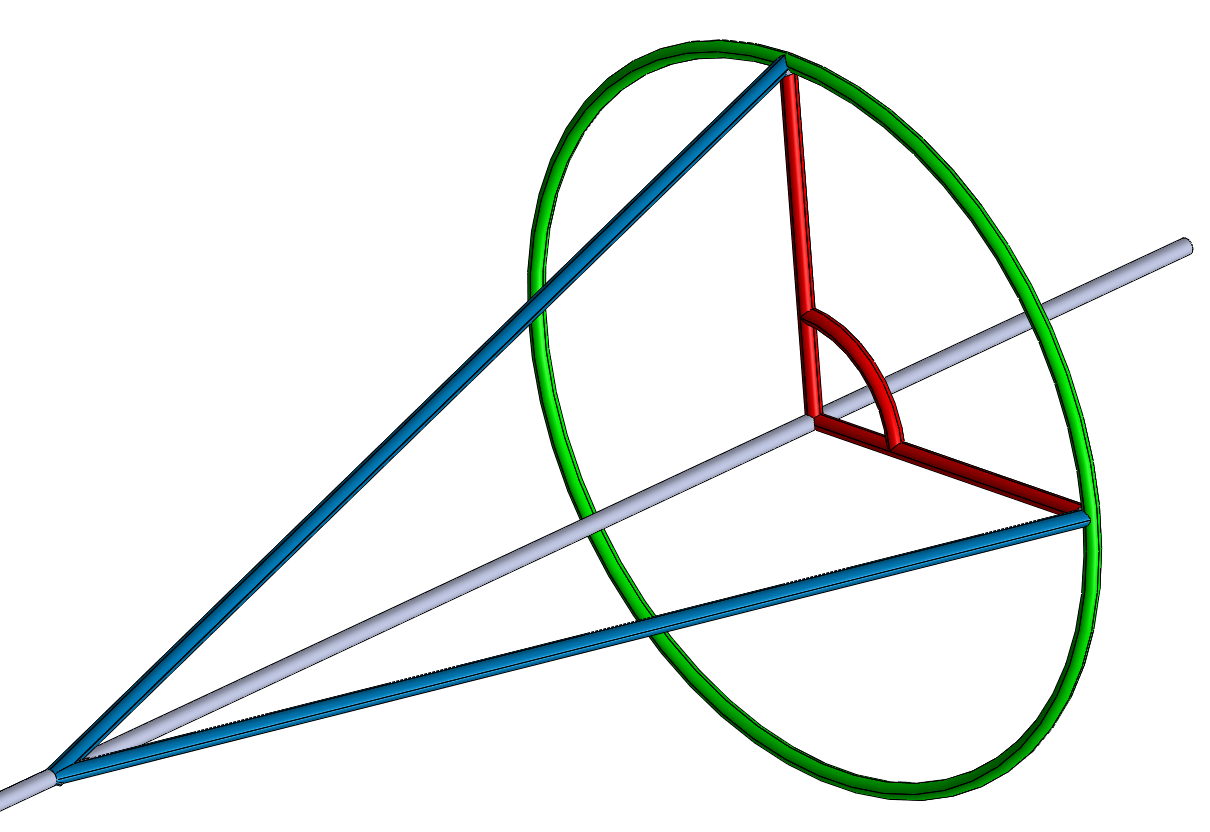
\includegraphics[width=0.8\textwidth]{子问题1.png}
        \[
            \mathrm{e}^{\hat{\xi}\theta}p = q
        \]
        \column{0.30\textwidth}
        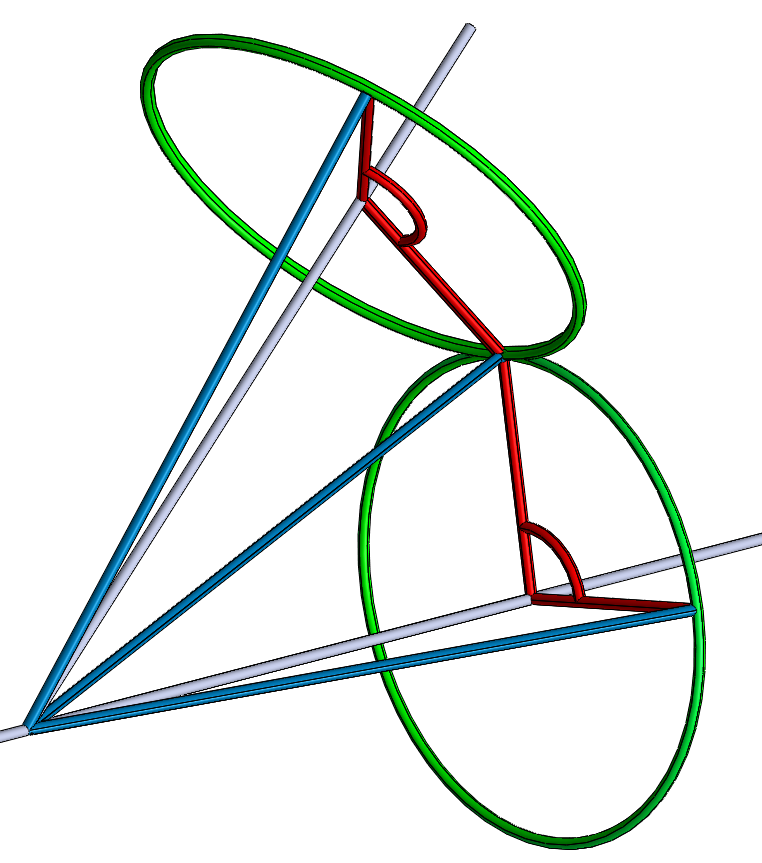
\includegraphics[width=0.8\textwidth]{子问题2.png}
        \[
            \mathrm{e}^{\hat{\xi}_1\theta_1}\mathrm{e}^{\hat{\xi}_2\theta_2}p = q
        \]
        \column{0.30\textwidth}
        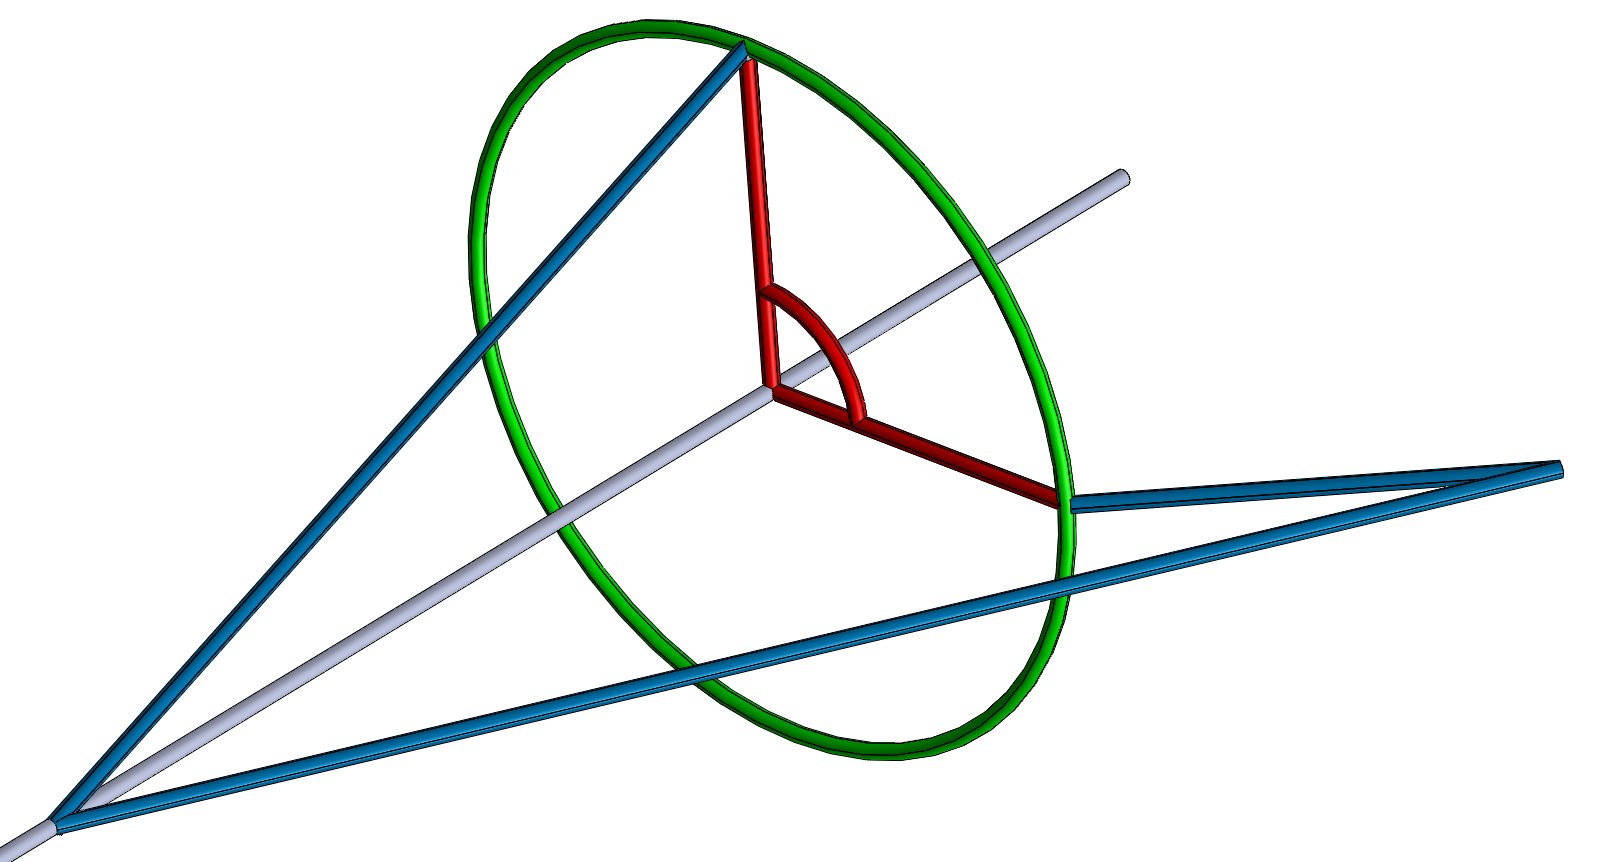
\includegraphics[width=0.8\textwidth]{子问题3.png}
        \[
            \Vert q - \mathrm{e}^{\hat{\xi}\theta}p \Vert = \delta
        \]
    \end{columns}
\end{frame}

%------------------------------------------------

\subsection{路径规划}

\begin{frame}
    \frametitle{路径规划:围绕最优搭建中心的分段直线}
    关键是确定“积木塔”的位置
    \begin{itemize}
        \item 与各个积木初始位置的距离之和最小
        \item 不可与积木初始位置重叠
    \end{itemize}
    \[
        \begin{aligned}
                 &  &  & p=[x,y,z,r,p,y]^T,\quad f(p) = \sum_{i=1}^N \Vert p-q_i \Vert \\
            s.t. &  &  & \Vert p-q_i \Vert \geq k                                      \\
            \min &  &  & f(p)
        \end{aligned}
    \]
    \begin{itemize}
        \item 含简单约束的凸优化问题,用数值方法求解
        \item 自行编写的算法时间复杂度为\(O(MN^2)\) \par \(M\)为搜索范围,\(N\)为物体数目。
    \end{itemize}
    % \begin{semiverbatim}
    % \textcolor{blue}{void} \textcolor{gray}{GeometricMedian}(\textcolor{blue}{const} \textcolor{orange}{vector<Vector2d>} \textcolor{blue}{\&}\textcolor{gray}{points},
    %                     \textcolor{orange}{Vector2d} \textcolor{blue}{\&}\textcolor{gray}{center}, 
    %                     \textcolor{blue}{double \&}\textcolor{gray}{min\_dist},
    %                     \textcolor{blue}{const double \&}\textcolor{gray}{forbidden\_zone\_radius},
    %                     \textcolor{blue}{const double \&}\textcolor{gray}{lower\_limit});
    % \end{semiverbatim}
\end{frame}

%------------------------------------------------

\subsection{轨迹规划}

\begin{frame}
    \frametitle{轨迹规划:操作空间,梯形速度}
    \[
        \vec x(n+1)- \vec x(n) = \left\{\begin{aligned}
             & \dfrac{1}{2} a_{acc} \vec k t_s^2(2n+1)                      &  & 0<n<N_{acc}       \\
             & v\vec kt_s                                                   &  & N_{acc}<n<N_{dec} \\
             & v \vec k t_s-\frac{1}{2} a_{dec} \vec k t_s^2(2n+1-2N_{dec}) &  & N_{dec}<n<N
        \end{aligned}\right.
    \]
    \centering
    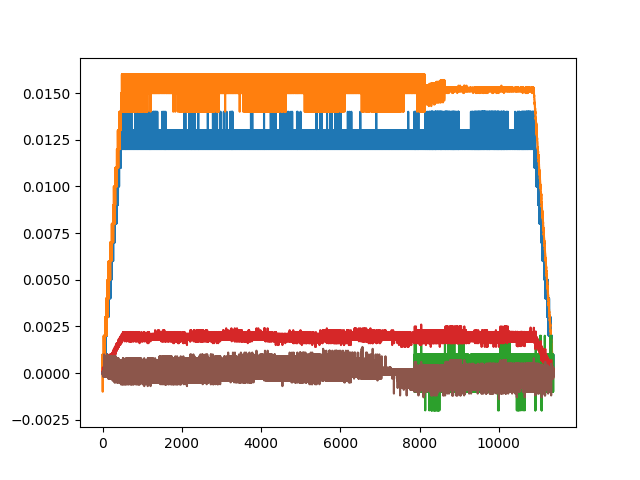
\includegraphics[scale=0.32]{轨迹规划.png}
\end{frame}

%------------------------------------------------

\section{软件系统}

\subsection{系统设计}

\begin{frame}
    \frametitle{系统设计:UML数据流图}
    \centering
    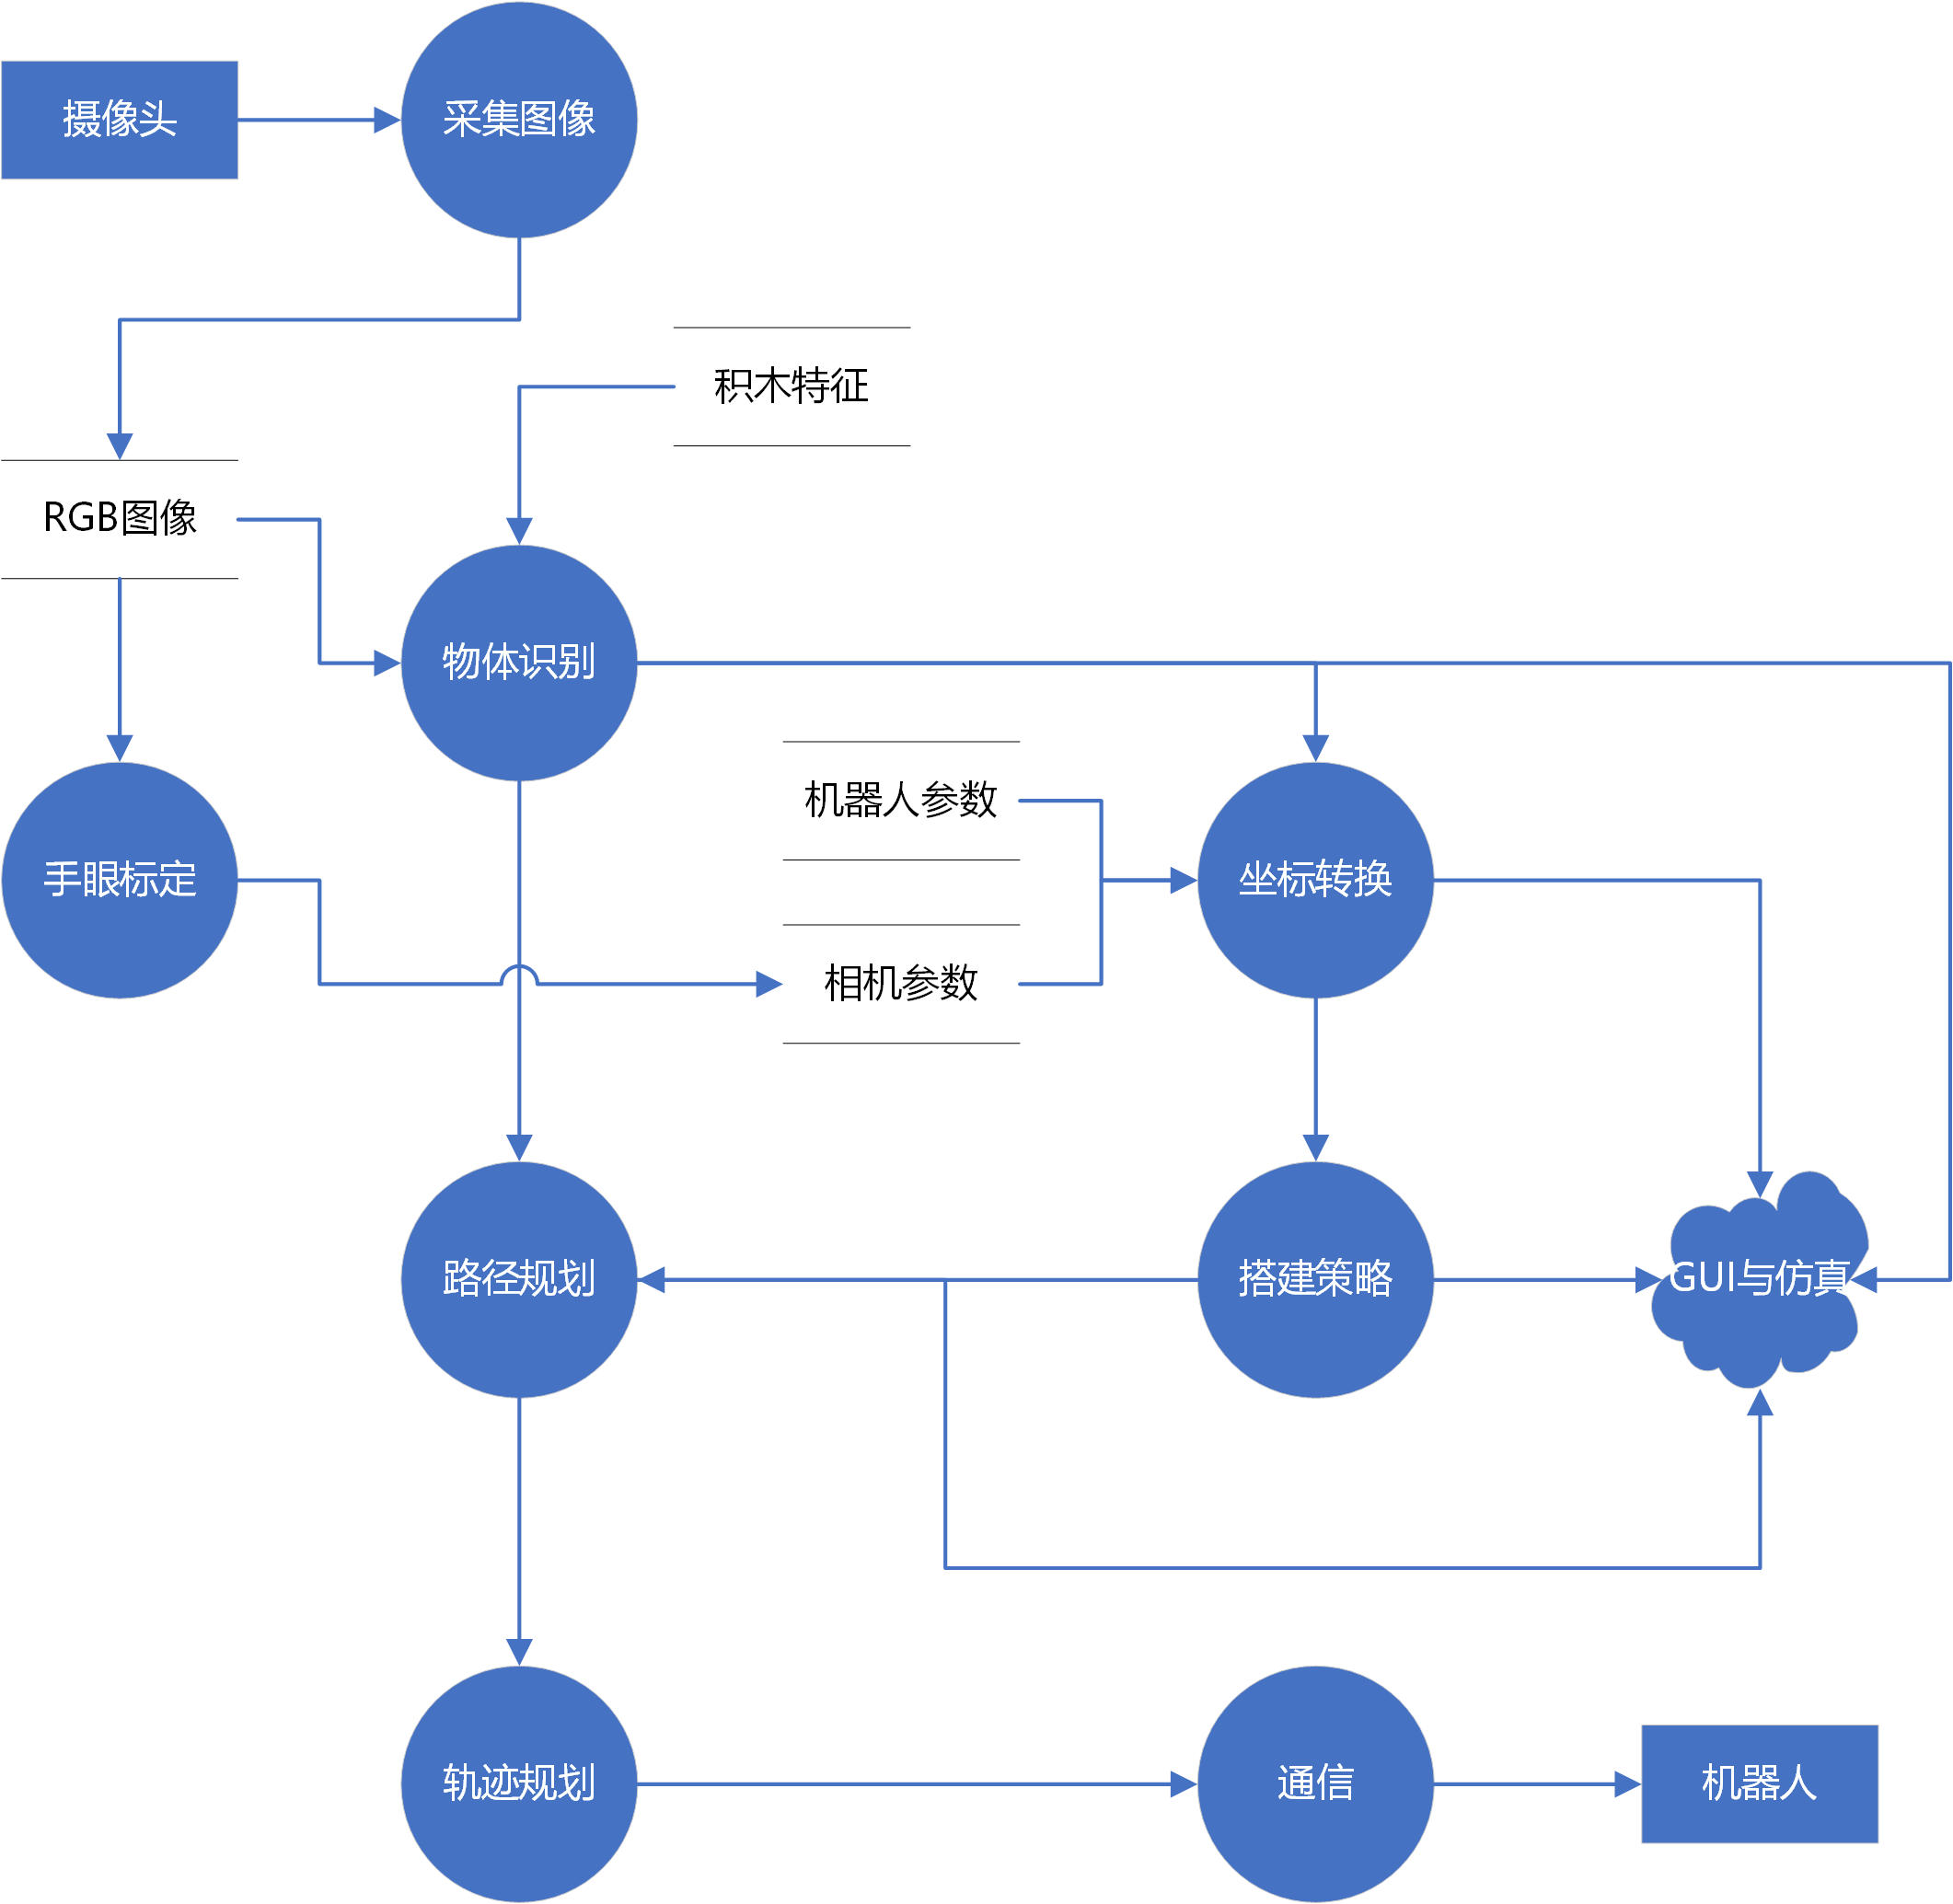
\includegraphics[scale=0.42]{UML数据流图.png}
\end{frame}

%------------------------------------------------

\begin{frame}
    \frametitle{系统设计:UML类图}
    \centering
    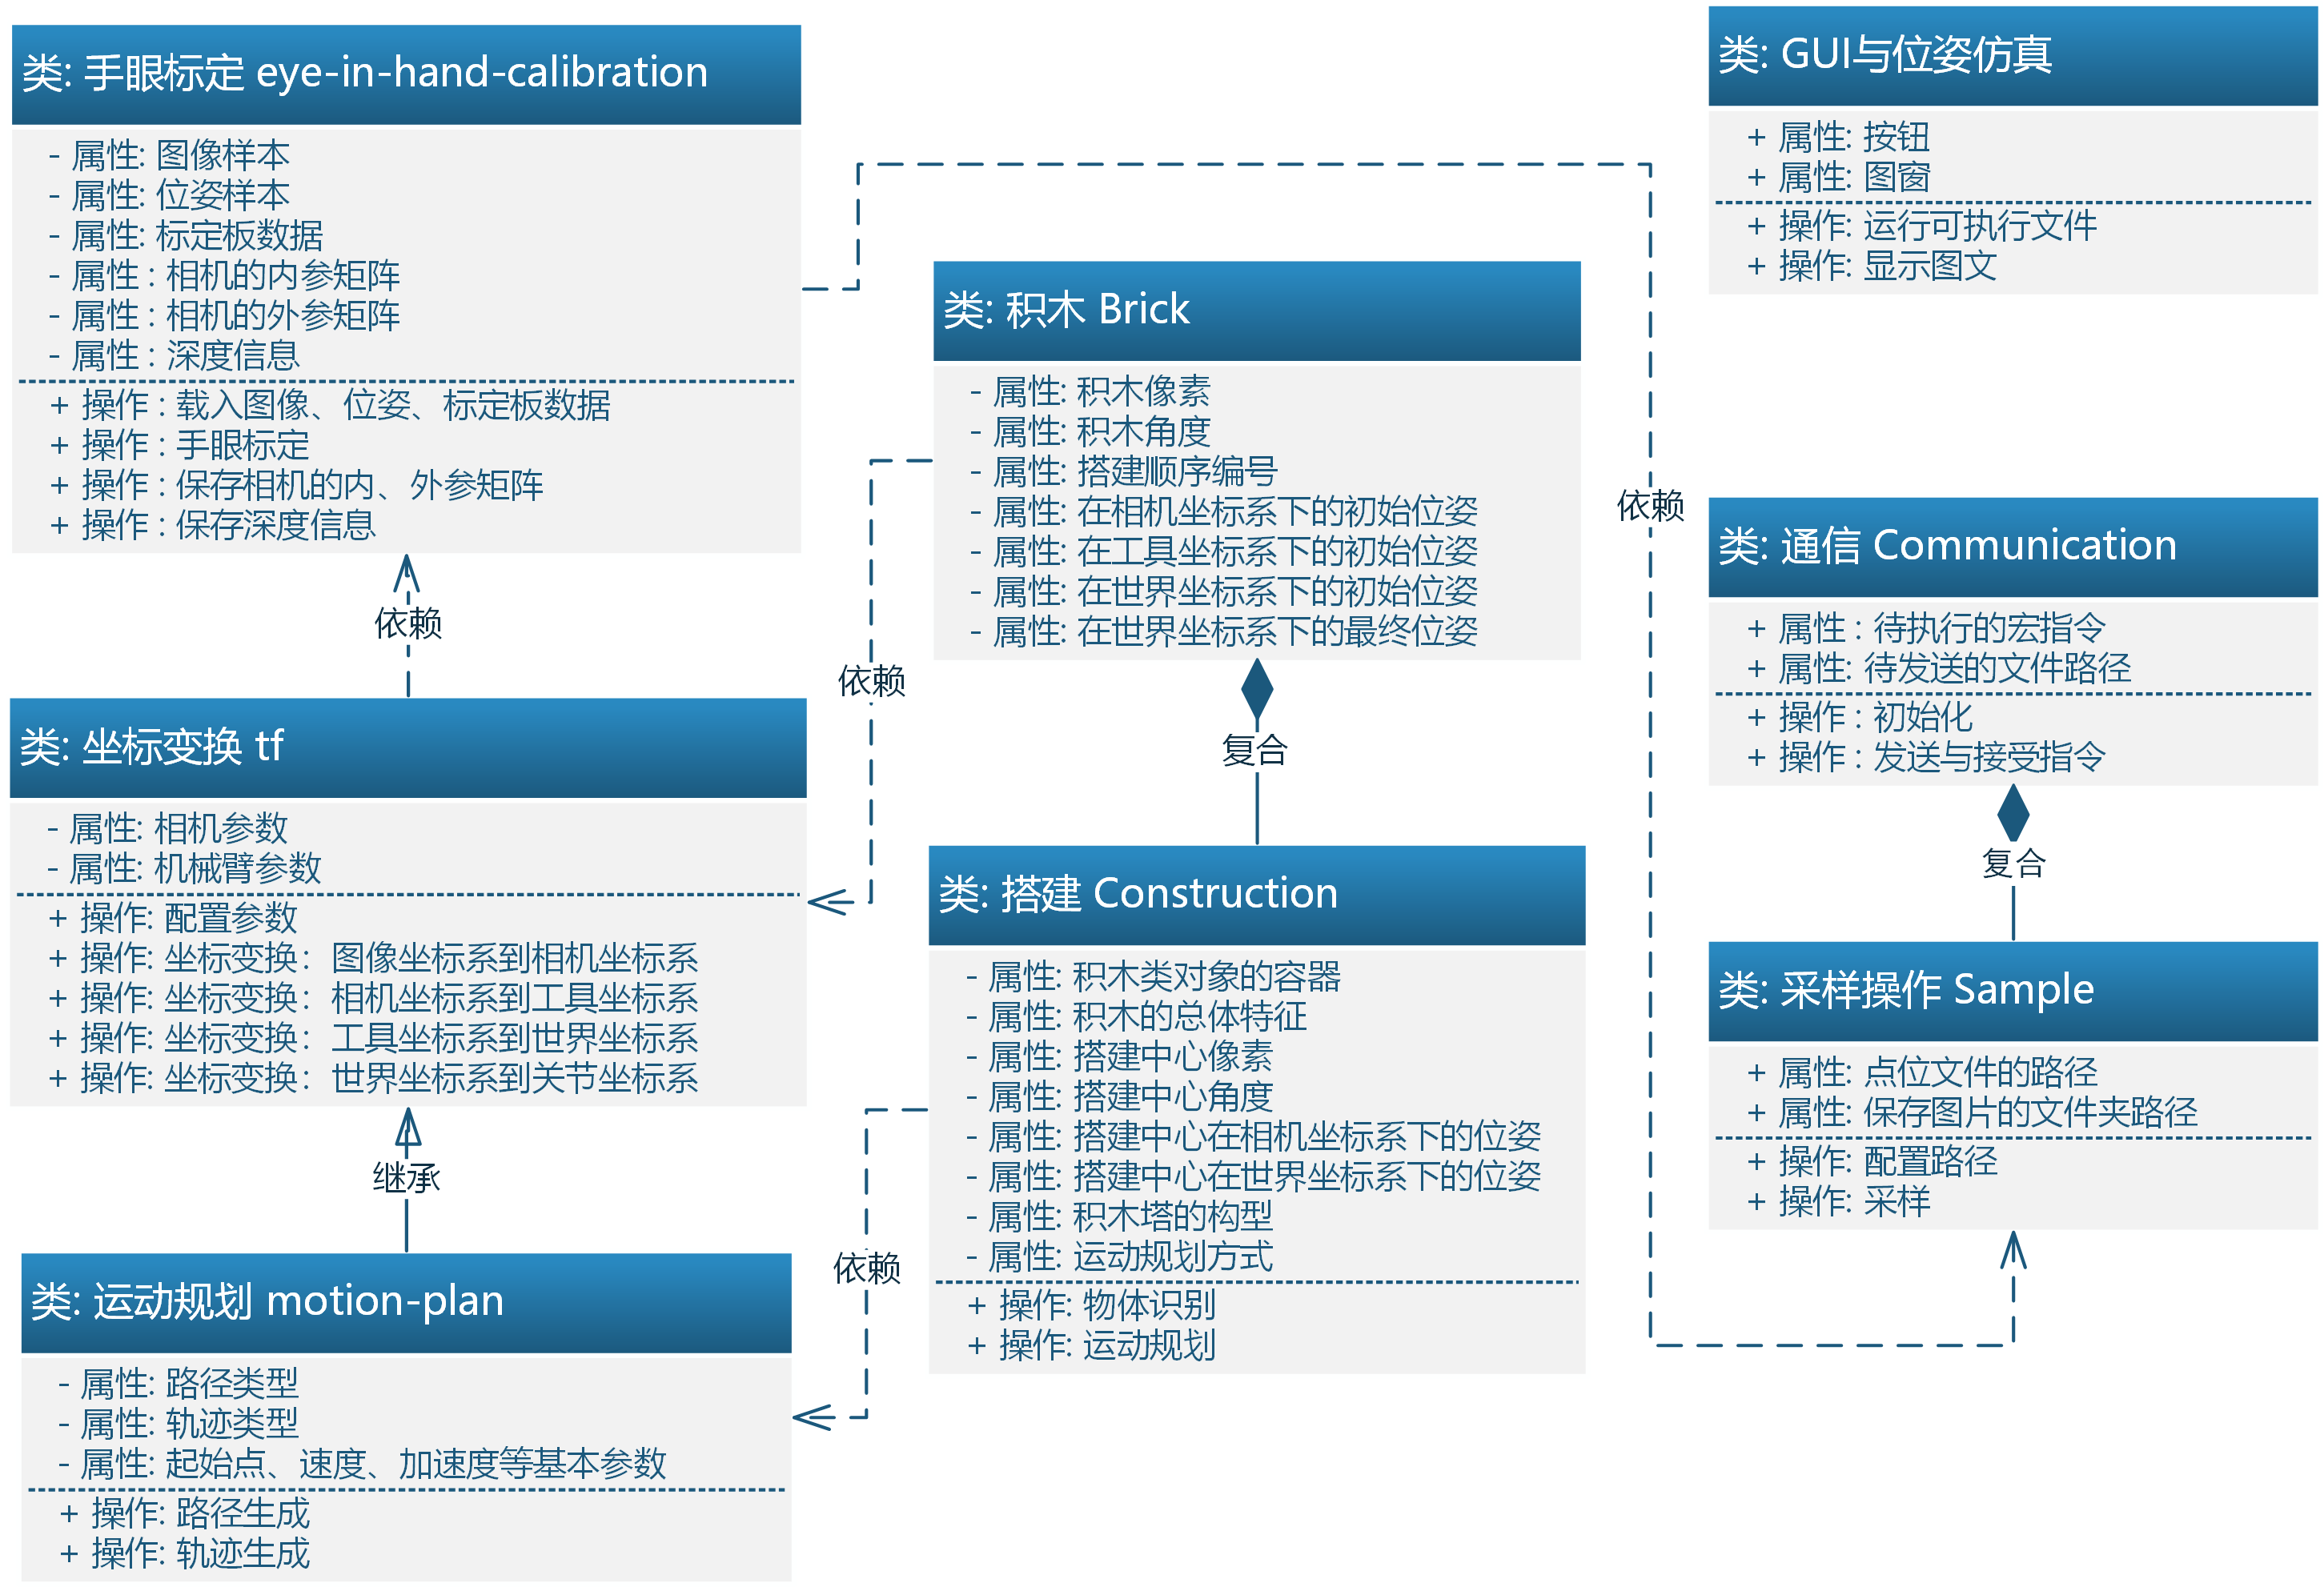
\includegraphics[scale=0.4]{UML类图.png}
\end{frame}

%------------------------------------------------

\subsection{工程实现}

\begin{frame}
    \frametitle{工程实现}
    \centering
    \begin{columns}[onlytextwidth,T]
        \column{\dimexpr\linewidth-40mm-5mm}
        \centering
        \begin{itemize}
            \item C++17编写,MinGW g++构建;
            \item GUI与位姿仿真使用Python编写。
        \end{itemize}
        \vspace*{1cm}
        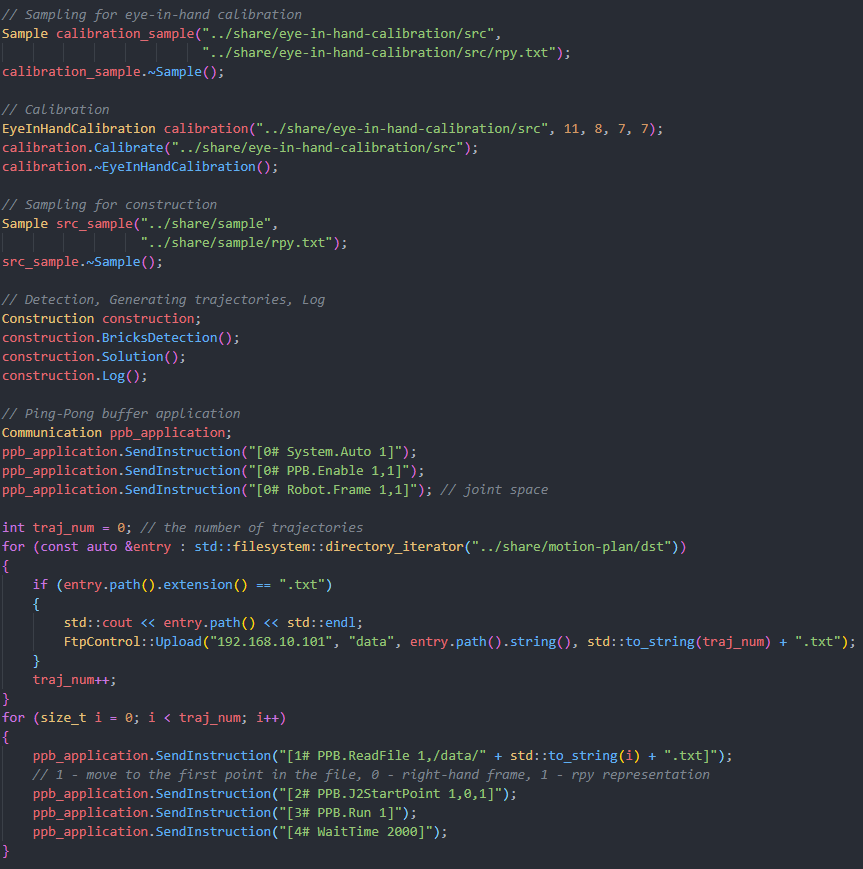
\includegraphics[scale=0.11]{主函数.png}\\
        \begin{center}
            主函数
        \end{center}
        \column{45mm}
        \centering
        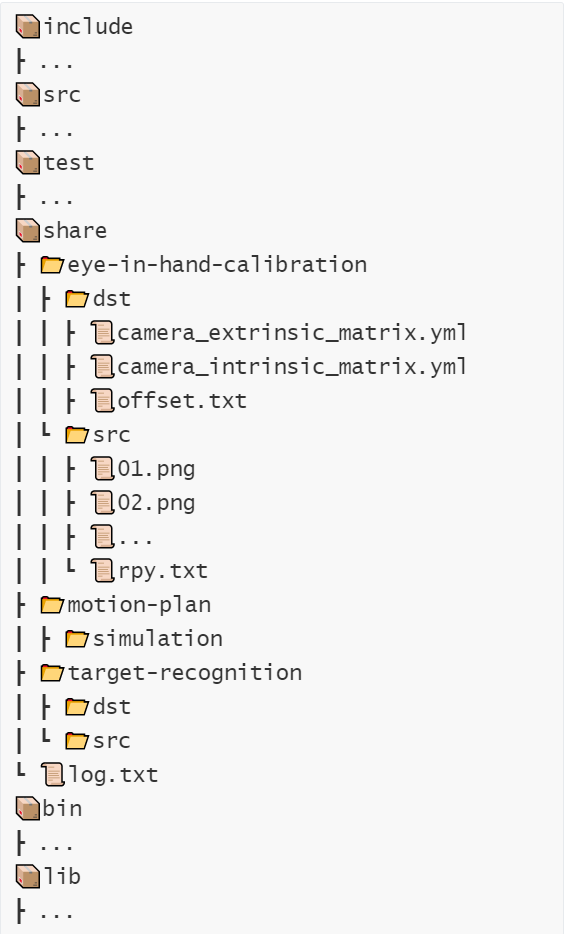
\includegraphics[scale=0.25]{file-tree.png}\\
        \begin{center}
            文件树
        \end{center}
    \end{columns}
\end{frame}

%------------------------------------------------

\subsection{成果演示}

\begin{frame}
    \frametitle{GUI演示:手眼标定}
    \centering
    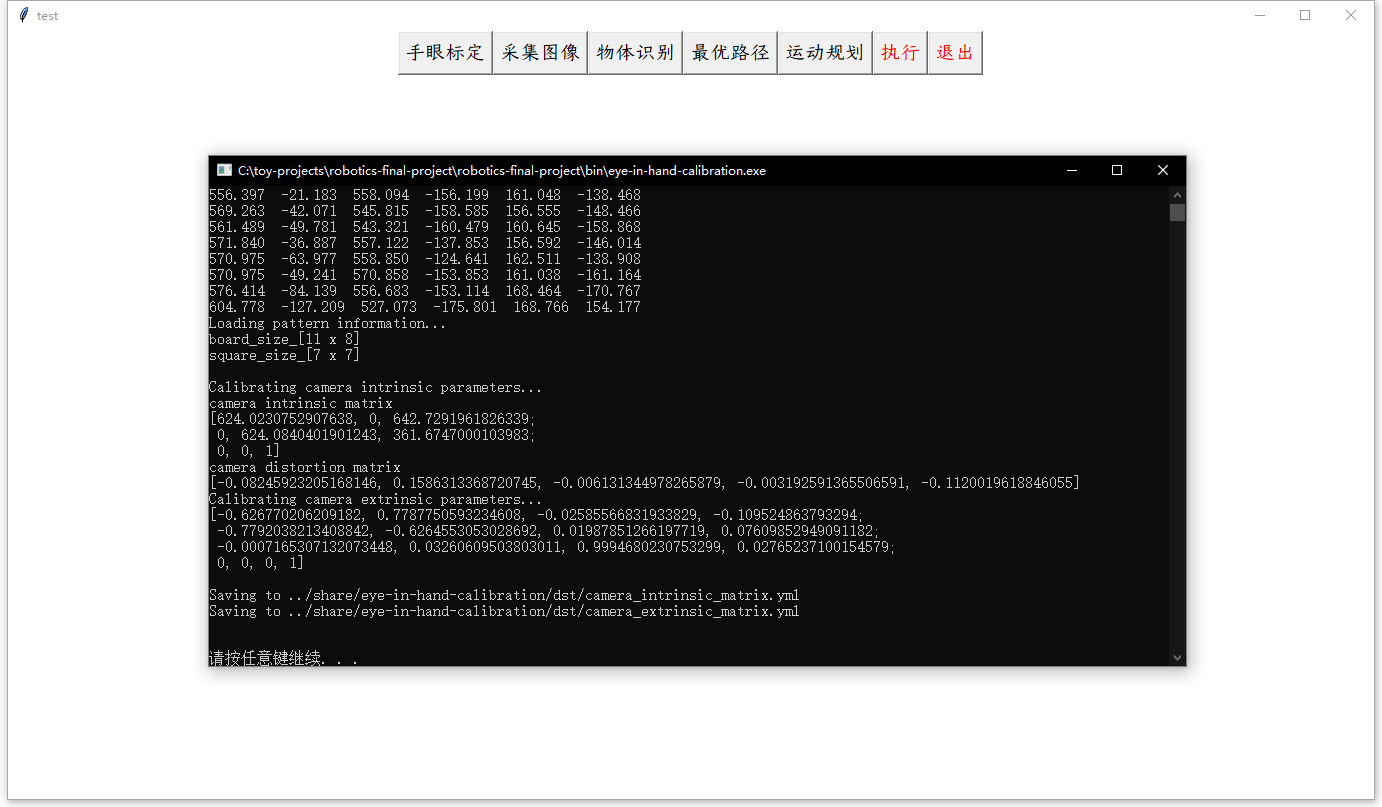
\includegraphics[scale=0.25]{手眼标定.png}
\end{frame}

\begin{frame}
    \frametitle{GUI演示:采集图像}
    \centering
    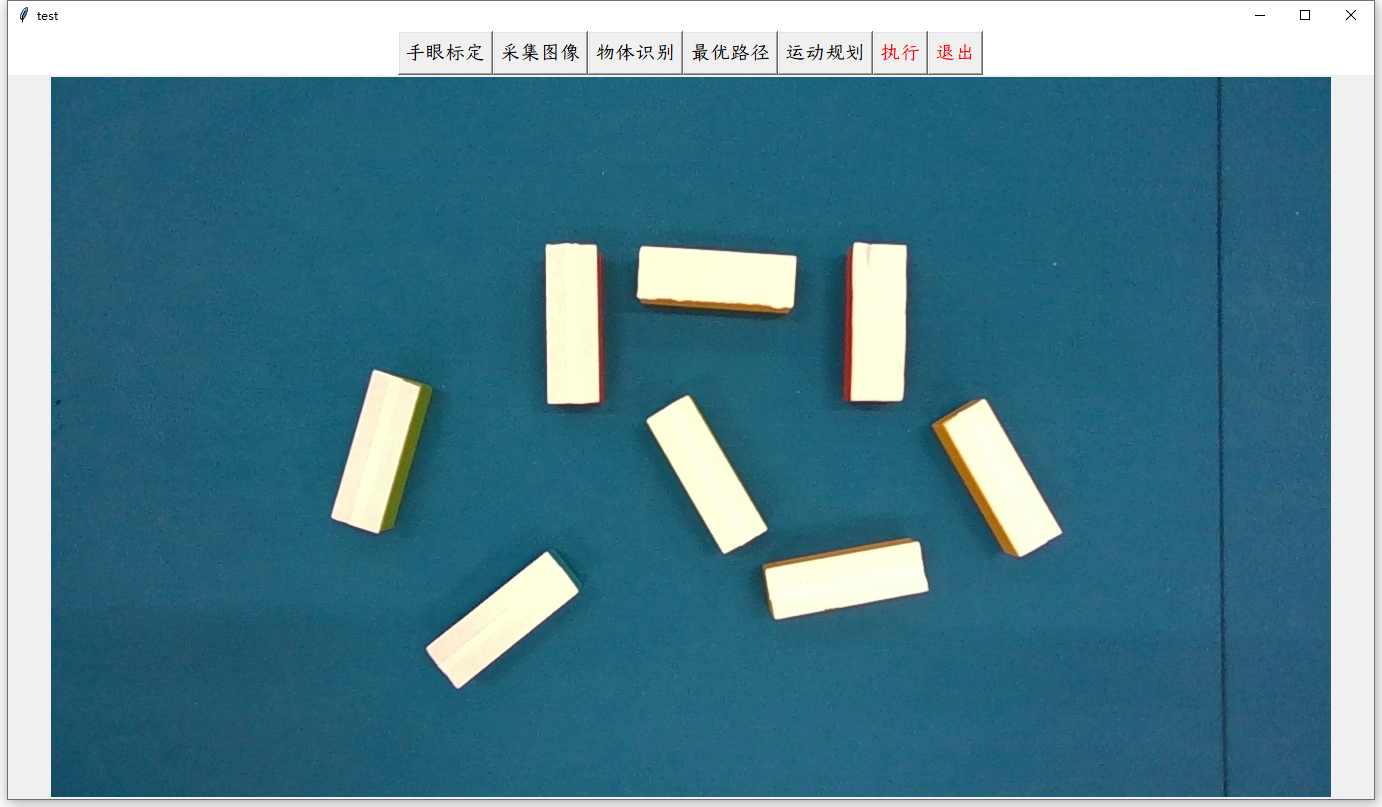
\includegraphics[scale=0.25]{采集图像.png}
\end{frame}

\begin{frame}
    \frametitle{GUI演示:物体识别}
    \centering
    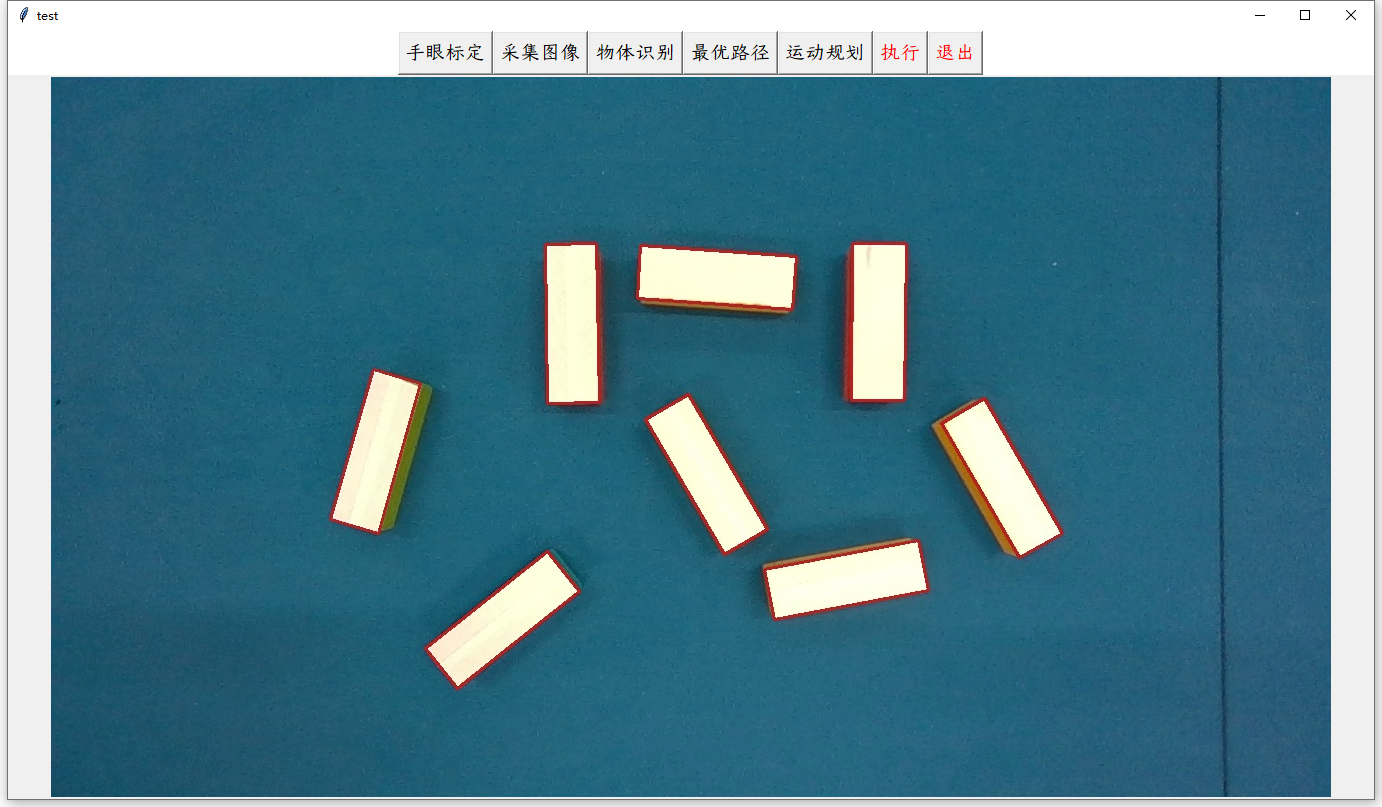
\includegraphics[scale=0.25]{物体识别.png}
\end{frame}

\begin{frame}
    \frametitle{GUI演示:最优搭建中心}
    \centering
    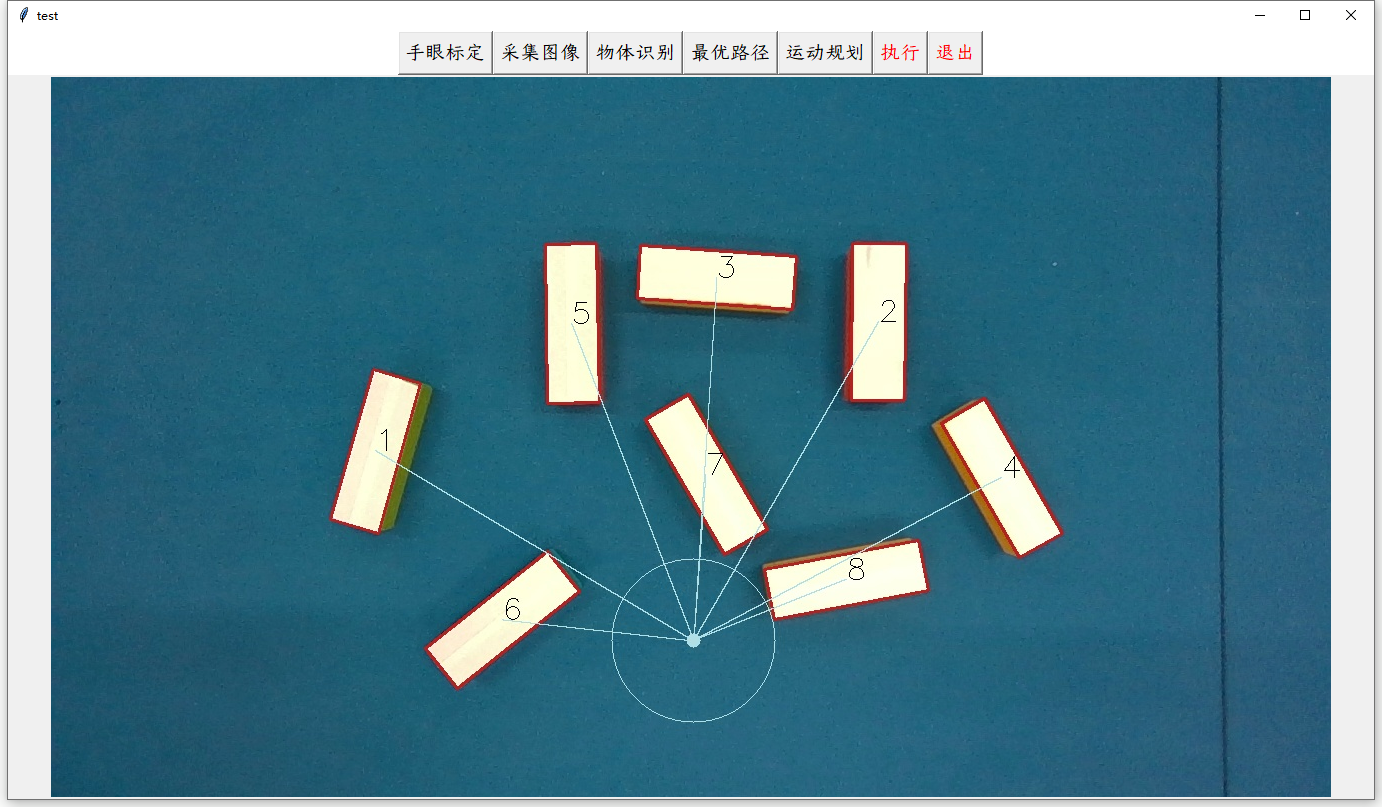
\includegraphics[scale=0.25]{路径规划.png}
\end{frame}

\begin{frame}
    \frametitle{GUI演示:路径规划}
    \centering
    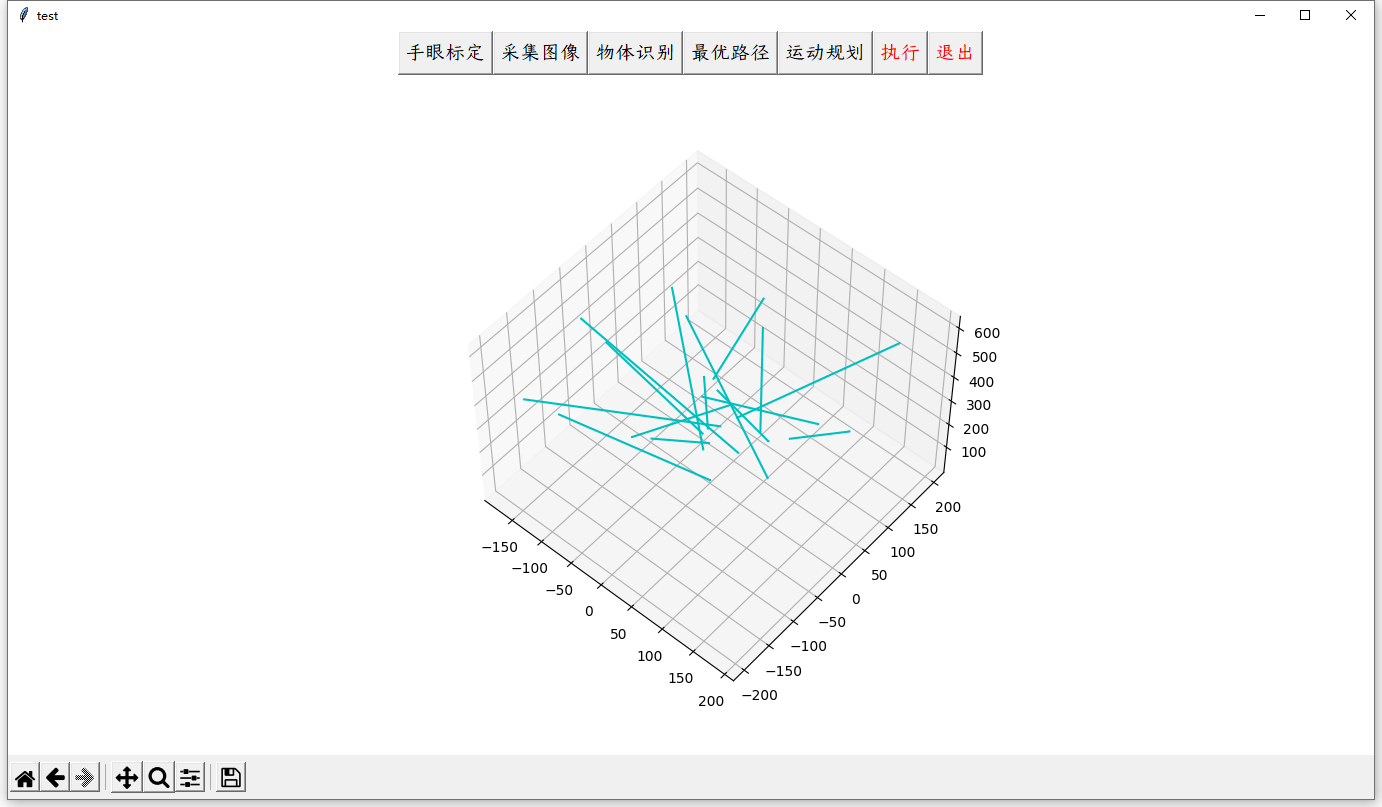
\includegraphics[scale=0.25]{运动规划_2.png}
\end{frame}

\begin{frame}
    \frametitle{GUI演示:起点终点的刚体位姿仿真}
    \centering
    \begin{columns}
        \column{\dimexpr\linewidth-60mm}
        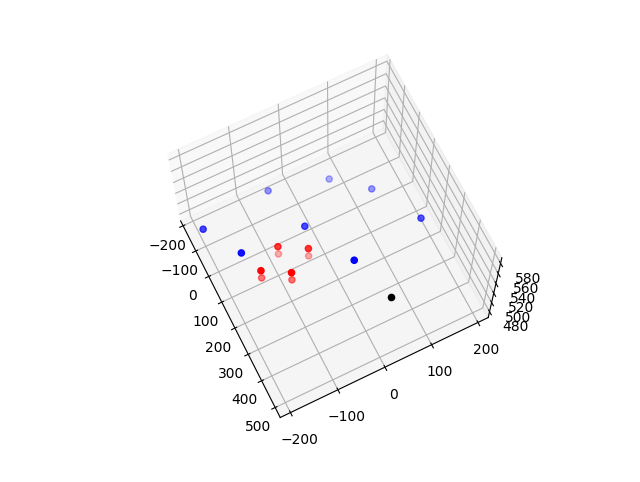
\includegraphics[width=48mm]{运动规划_3.png}
        \column{45mm}
        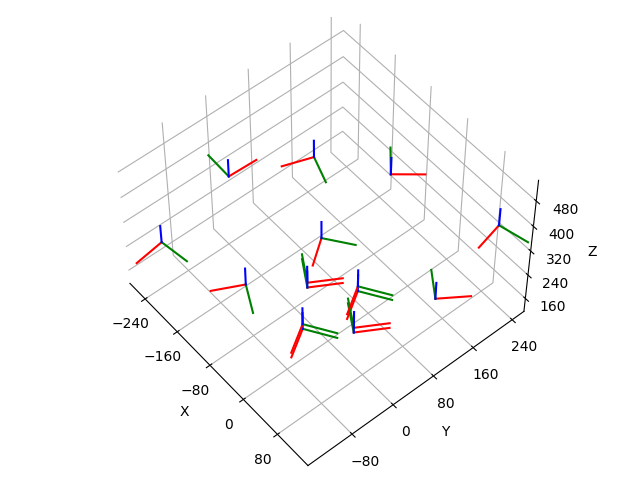
\includegraphics[width=45mm]{起点与终点的位姿仿真.png}
    \end{columns}
    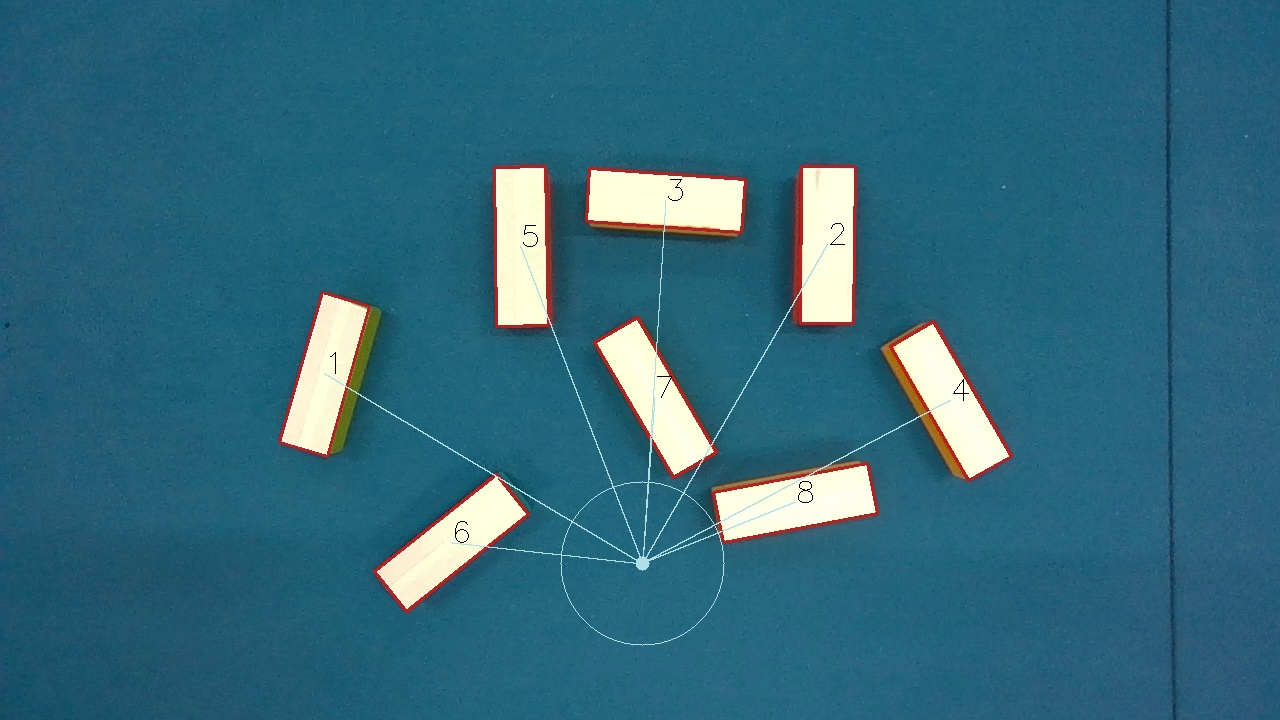
\includegraphics[scale=0.10]{img_strategy.jpg}
\end{frame}

%------------------------------------------------

\section{总结}

\begin{frame}
    \frametitle{总结}
    \begin{columns}
        \column{0.5\textwidth}
        \begin{center}
            特色
        \end{center}
        \begin{enumerate}
            \item 面向对象的系统设计与实现;
            \item 路径规划:凸优化;
            \item 刚体位姿的简单可视化仿真;
            \item 图形用户界面;
        \end{enumerate}
        \column{0.5\textwidth}
        \begin{center}
            待改进
        \end{center}
        \begin{enumerate}
            \item 优化轨迹规划,物体识别等方法;
            \item 利用Realsense相机的深度信息提升精度;
            \item 完善仿真功能;
            \item 项目的可维护性;
            \item 跨平台;
        \end{enumerate}
    \end{columns}
\end{frame}

%------------------------------------------------

\begin{frame}
    \Huge{\centerline{The End}}
\end{frame}

%------------------------------------------------

\end{document}